\documentclass{standalone}
\usepackage{tikz}
\begin{document}
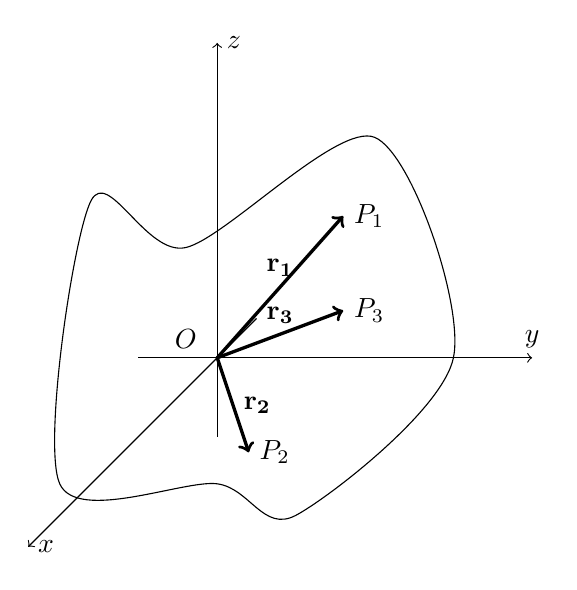
\begin{tikzpicture}[scale=2]
    \coordinate(O)at(0,0);
    \draw[->](-0.5,0)--(2,0)node[above]{$y$};
    \draw[->](0,-0.5)--(0,2)coordinate(z)node[right]{$z$};
    \draw[->](0.25,0.25)--(-1.2,-1.2)node[right]{$x$}; 
    \node[above]at(-0.2,0){$O$};
    
    \draw[->, very thick](O)--(0.8,0.9)node[midway, above]{$\mathbf{r_1}$}node[right]{$P_1$};
    \draw[->, very thick](O)--(0.2,-0.6)node[midway, right]{$\mathbf{r_2}$}node[right]{$P_2$};
    \draw[->, very thick](O)--(0.8,0.3)node[midway, above]{$\mathbf{r_3}$}node[right]{$P_3$};

    \draw[-]plot[smooth cycle]coordinates{(1.5,0)(1,1.4)(-0.2,0.7)(-0.8,1)(-1,-0.8)(0,-0.8)(0.5,-1)};
\end{tikzpicture}
\end{document}